\chapter{Estado del Arte}
\label{cap:estadoDeLaCuestion}

\begin{resumen}
	En este capítulo revisaremos las principales bases de datos disponibles y examinaremos los métodos de \emph{Deep Learning} más relevantes para su análisis, destacando el modelo de \cite{ribeiro} como punto de referencia en el estado del arte. Por último, revisaremos el significado de explicabilidad en el ámbito de la IA y mencionaremos algunos trabajos que tratan temas relacionados con este.
\end{resumen}

\section{Bases de datos}

Para entrenar modelos que permitan analizar automáticamente las señales de un ECG es esencial la disponibilidad de una gran cantidad de ECGs. En esta sección se revisan brevemente algunas colecciones de ECGs ampliamente utilizadas en el ámbito de la investigación y se presentan en detalle las características de PTB-XL, la base de datos elegida para la realización de este trabajo.

\subsection{Bases de datos disponibles}
\label{subsec:databases}
Como queremos comparar el rendimiento de varias modificaciones de un modelo ya existente, lo ideal sería poder trabajar con la misma base de datos con la que se entrenó el modelo de Ribeiro. Esta base de datos es CODE \citep{code}, pero no es pública, por lo que esto no es una opción.

Existe una versión pública reducida de esta base de datos llamada CODE-15 \citep{code15}, que tiene alrededor de 350000 casos. No obstante, no podemos comparar un modelo entrenado con los datos de CODE-15 con otro entrenado con los de  CODE, porque la ventaja en el conjunto de datos de entrenamiento haría imposible comparar la eficiencia de manera equitativa. Por ello, vamos a volver a entrenar el \emph{gold standard} con una base de datos pública, PTB-XL \citep{ptbxldb}. Esta base de datos cuenta con unos 22000 casos de prueba, pero todos estos casos están con el mismo formato, por lo que el procesamiento de los mismos será más sencillo. Adicionalmente, dado que el objetivo es comparar distintas modificaciones del modelo para evaluar si mejora el rendimiento, es mucho más importante emplear bases de datos uniformes y poder realizar más entrenamientos que usar una base de datos más grande, lo que incrementaría significativamente el tiempo de entrenamiento.

\subsection{PTB-XL}
La base de datos PTB-XL es un conjunto de registros de ECGs de 12 derivaciones que reune información de miles de pacientes, con edades y condiciones de salud variadas \citep{ptbxlart}. Se caracteriza por:

	\subsubsection{Número de muestras}
	 La base de datos incluye 21799 registros. Cada registro tiene una duración de 10 segundos y está disponible a una frecuencia de 100Hz y 500Hz. El hecho de que todos los registros sean uniformes facilita en gran medida el preprocesamiento de los datos.
	
	\subsubsection{Etiquetas clínicas}
	\label{subsec:anomalias}
	 Se proporciona un conjunto de anotaciones diagnósticas que abarcan una amplia serie de condiciones. Adicionalmente, se incluye un archivo en formato \emph{.csv} con información sobre cada condición.
	 
	 Todas las posibles anomalías de un ECG se agrupan en cuatro clases diferentes, con una clase adicional para los ECGs categorizados como normales. Las etiquetas son las siguientes:
	 
	 \begin{itemize}
	 	\item \textbf{Normal (NORM)}: Esta etiqueta significa que el ECG se categoriza como normal, y por tanto no tiene ninguna anomalía \footnote{Esto no significa que un ECG con esta etiqueta no pueda tener también otras etiquetas. Por como funciona el modelo, se decide para cada una de las 5 etiquetas la probabilidad de que pertenezca a esta, y luego (mediante un umbral de 0.5), se binariza la pertenencia a etiquetas. Esto hace que el modelo pueda etiquetar un mismo ECG como normal y con una anomalía, lo cuál no es intuitivo. Una posible línea de trabajo futuro es modificar esta etiqueta para que sea exclusiva, es decir, que solo se aplique si no coincide con ninguna anomalía.}
	 	
	 	\item \textbf{Infartos de miocardio (MI)}: Las anomalías en esta categoría presentan cambios similares a las STTC, pero su causa clínica es más específica.
	 	
	 	\item \textbf{Anomalías del segmento ST y onda T (STTC)}: Esta categoría incluye elevaciones o descensos anómalos del segmento ST, así como cambios en la morfología de la onda T, siempre que no puedan ser clasificados como infartos de miocardio.
	 	
	 		 	
	 	\item \textbf{Anomalías de la conducción (CD)}: Esta categoría se caracteriza por ensanchamientos en el complejo QRS o modificaciones de la progresión de las ondas en el trazado.

	 	\item \textbf{Hipertrofia (HYP)}: Esta categoría (que es la menos común) presenta alteraciones en la amplitud del complejo QRS o cambios en las ondas ST/T.	 	

	 \end{itemize}
	 
	 En la Figura \ref{fig:ecg_clases} podemos ver ECGs que presentan cada tipo de anomalía. Para una descripción detallada y exhaustiva de las anomalías cardíacas y su clasificación, el lector puede referirse a \textbf{Braunwald's Heart Disease: A Textbook of Cardiovascular Medicine} \cite{Mann2021}.
	 
	 \begin{figure}
	 	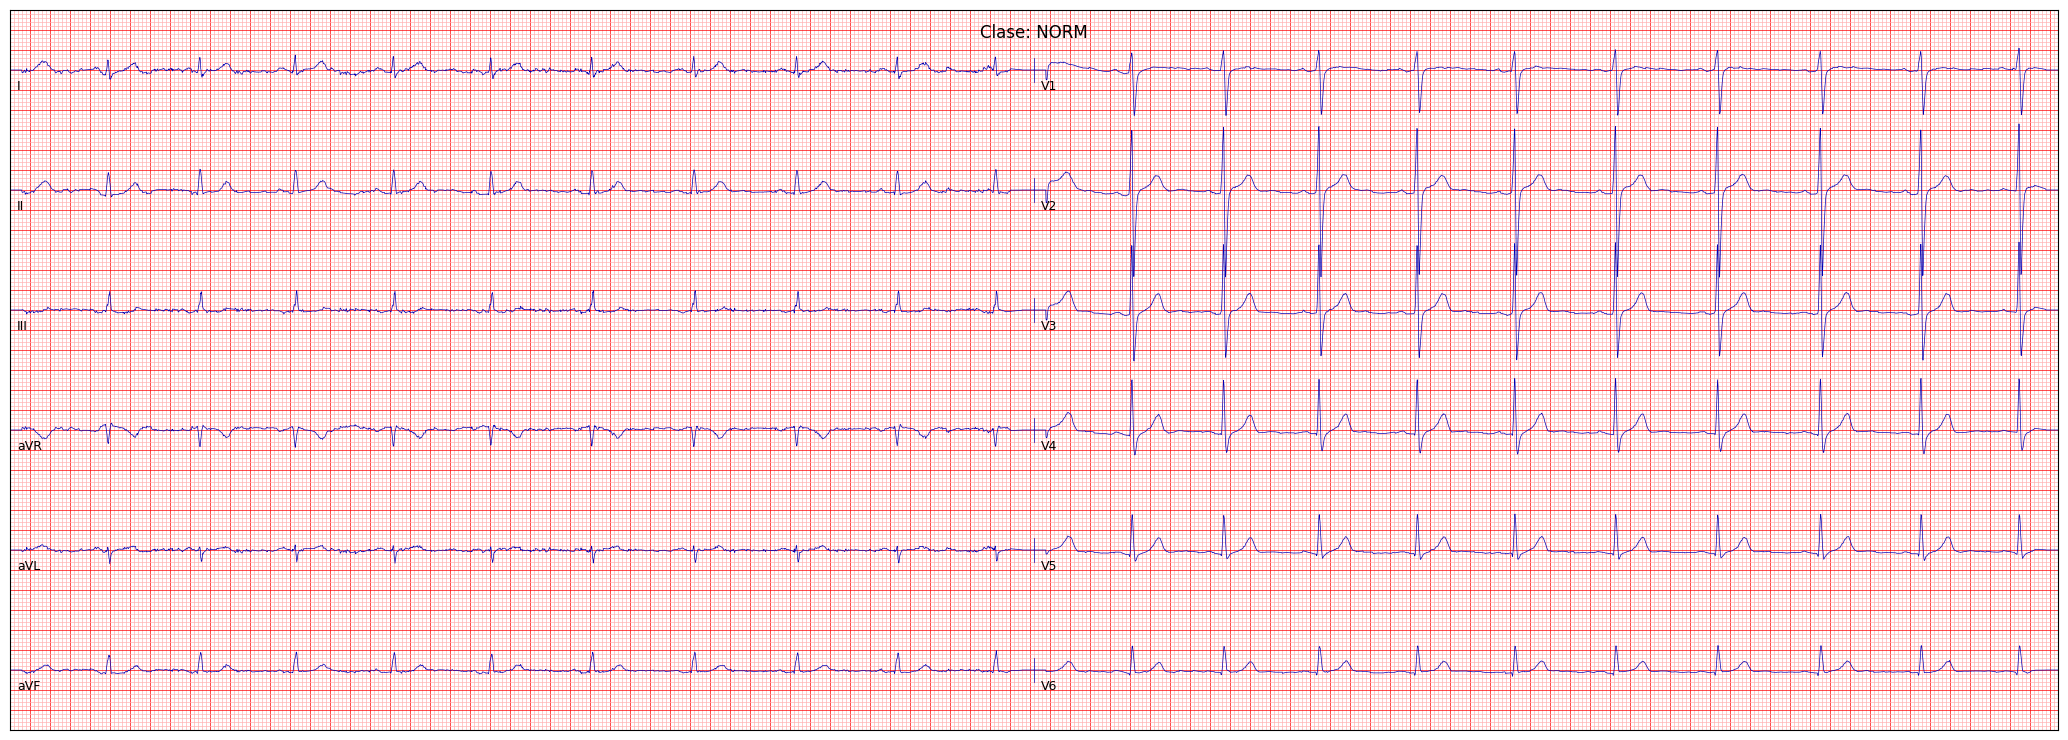
\includegraphics[width=0.9\textwidth]{Imagenes/Vectorial/ECG/NORM.png}
	 	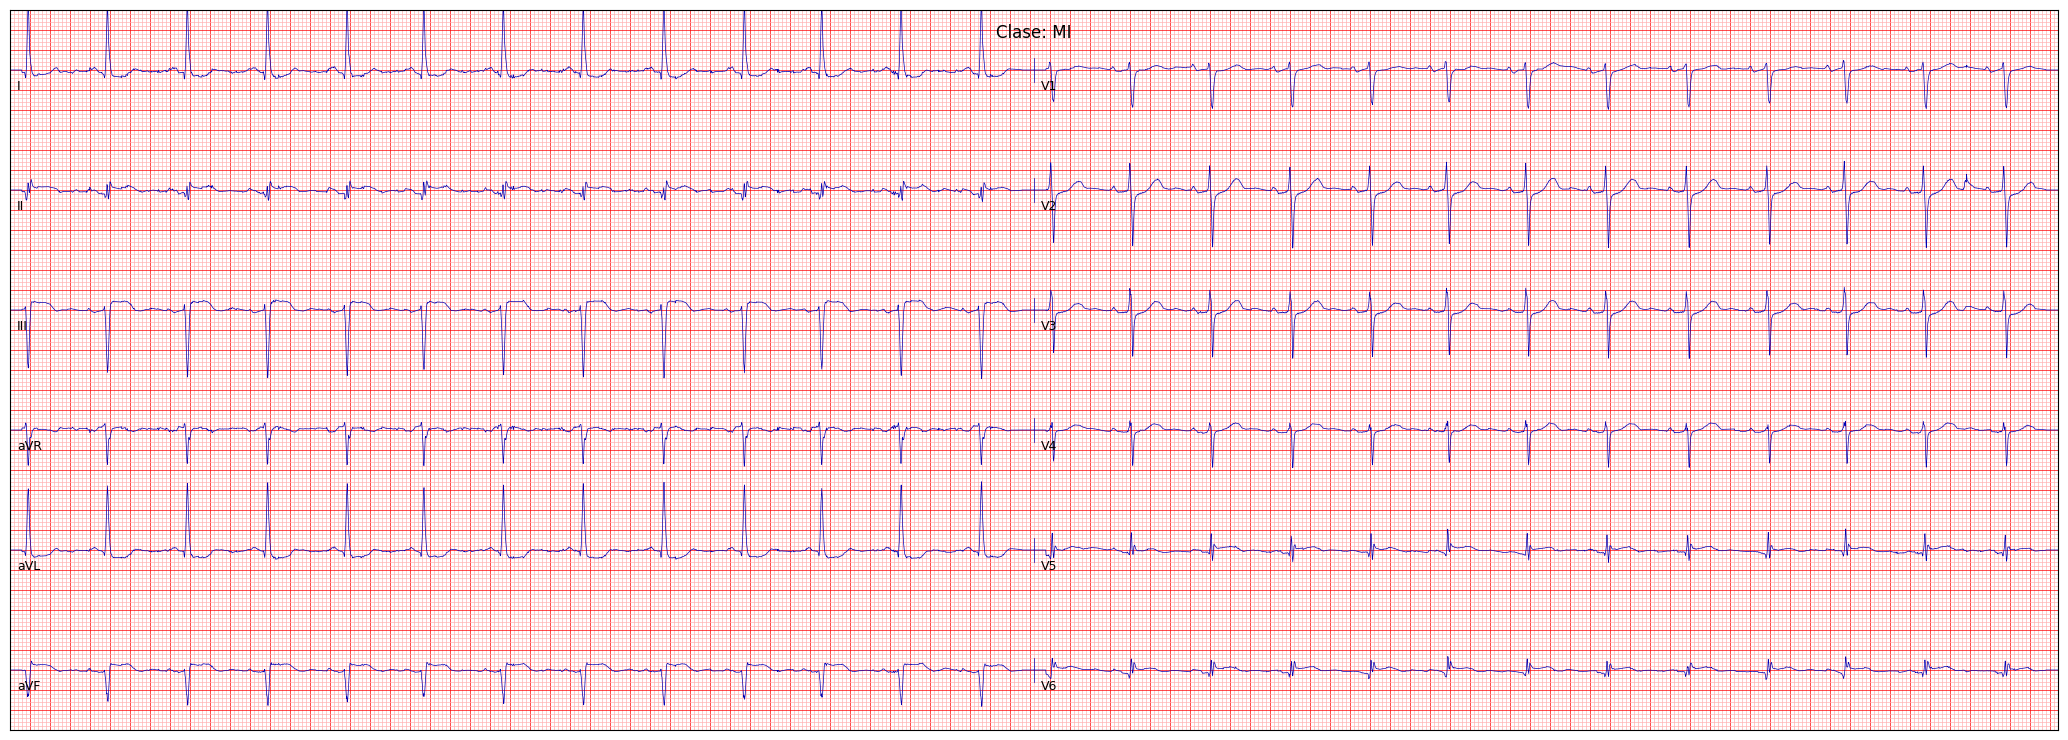
\includegraphics[width=0.9\textwidth]{Imagenes/Vectorial/ECG/MI.png}
	 	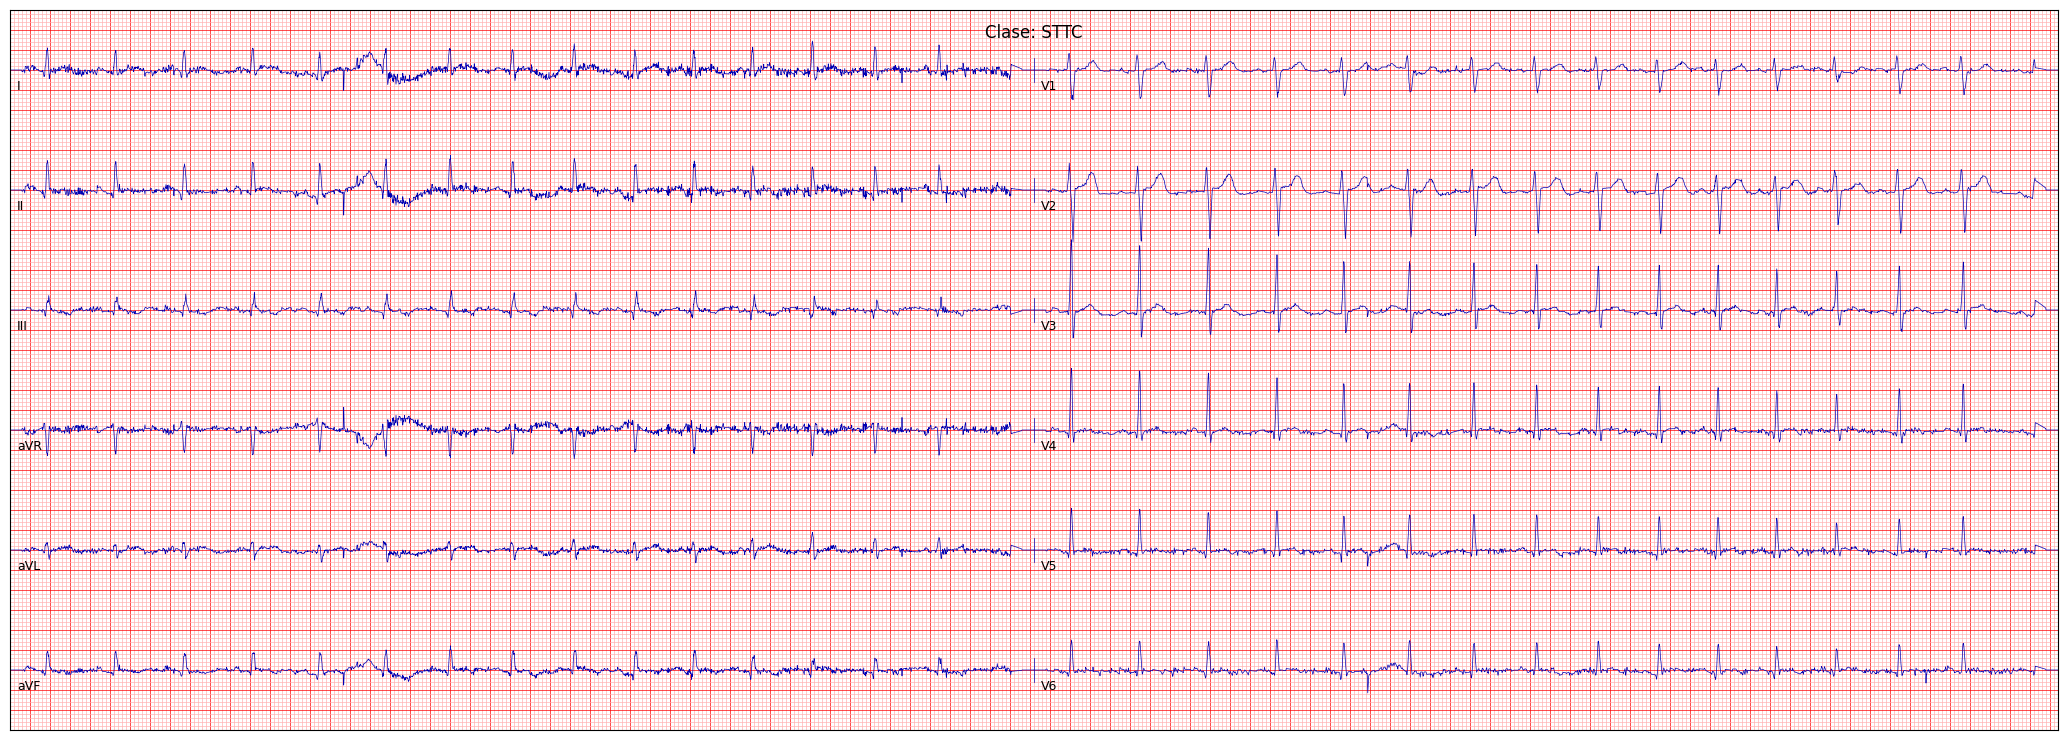
\includegraphics[width=0.9\textwidth]{Imagenes/Vectorial/ECG/STTC.png}
	 	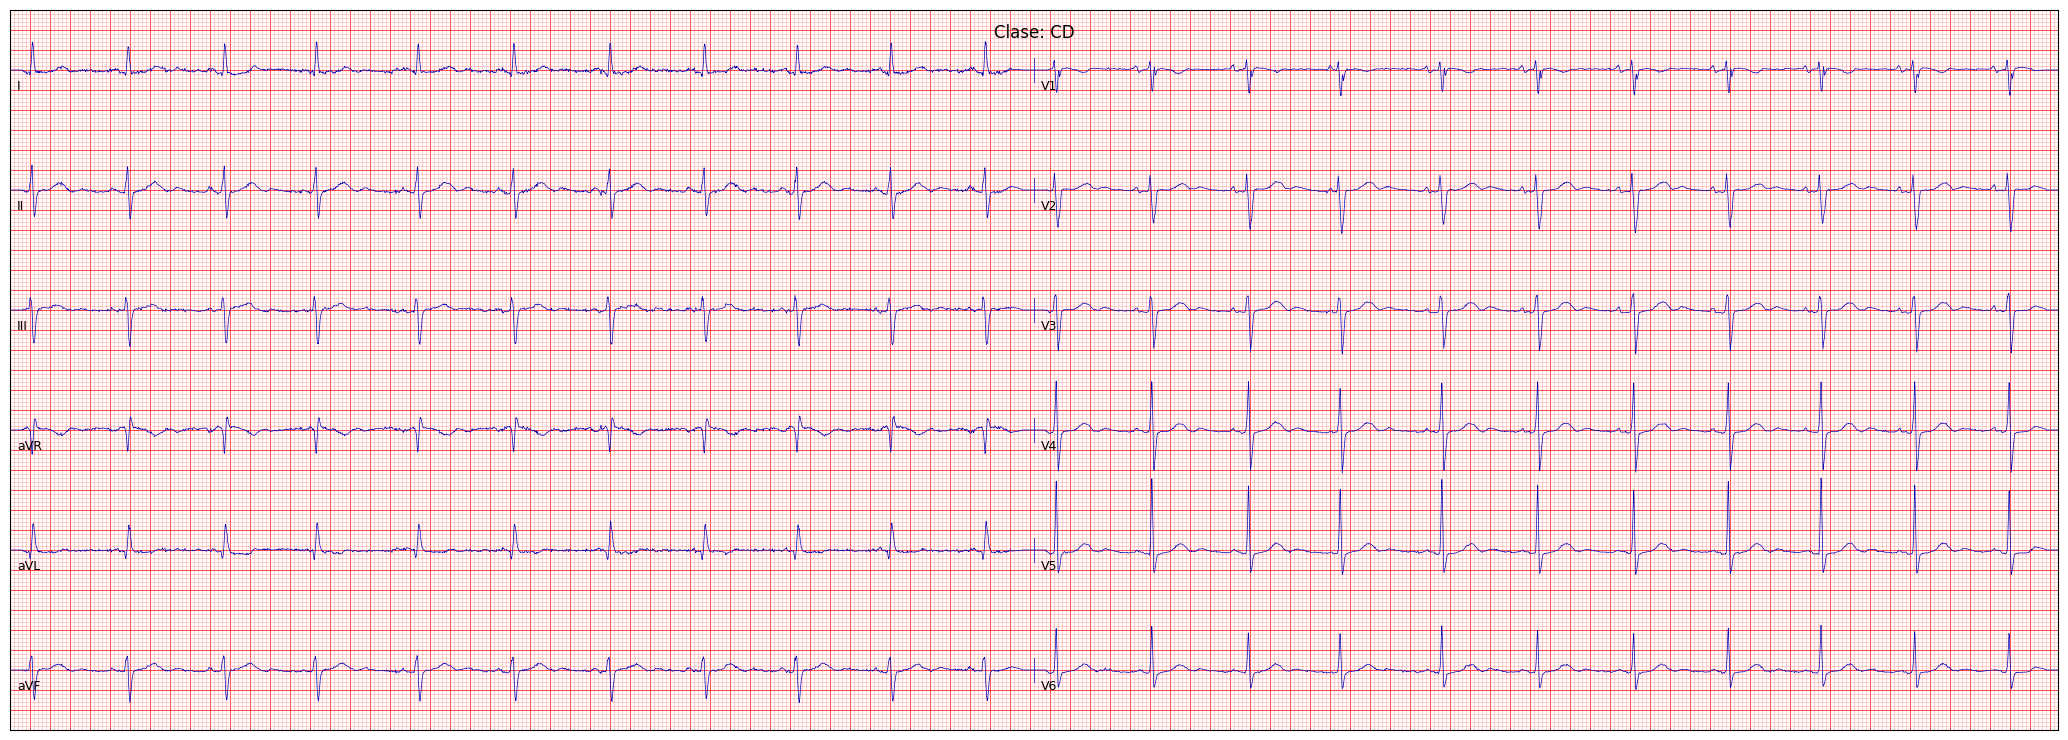
\includegraphics[width=0.9\textwidth]{Imagenes/Vectorial/ECG/CD.png}
	 	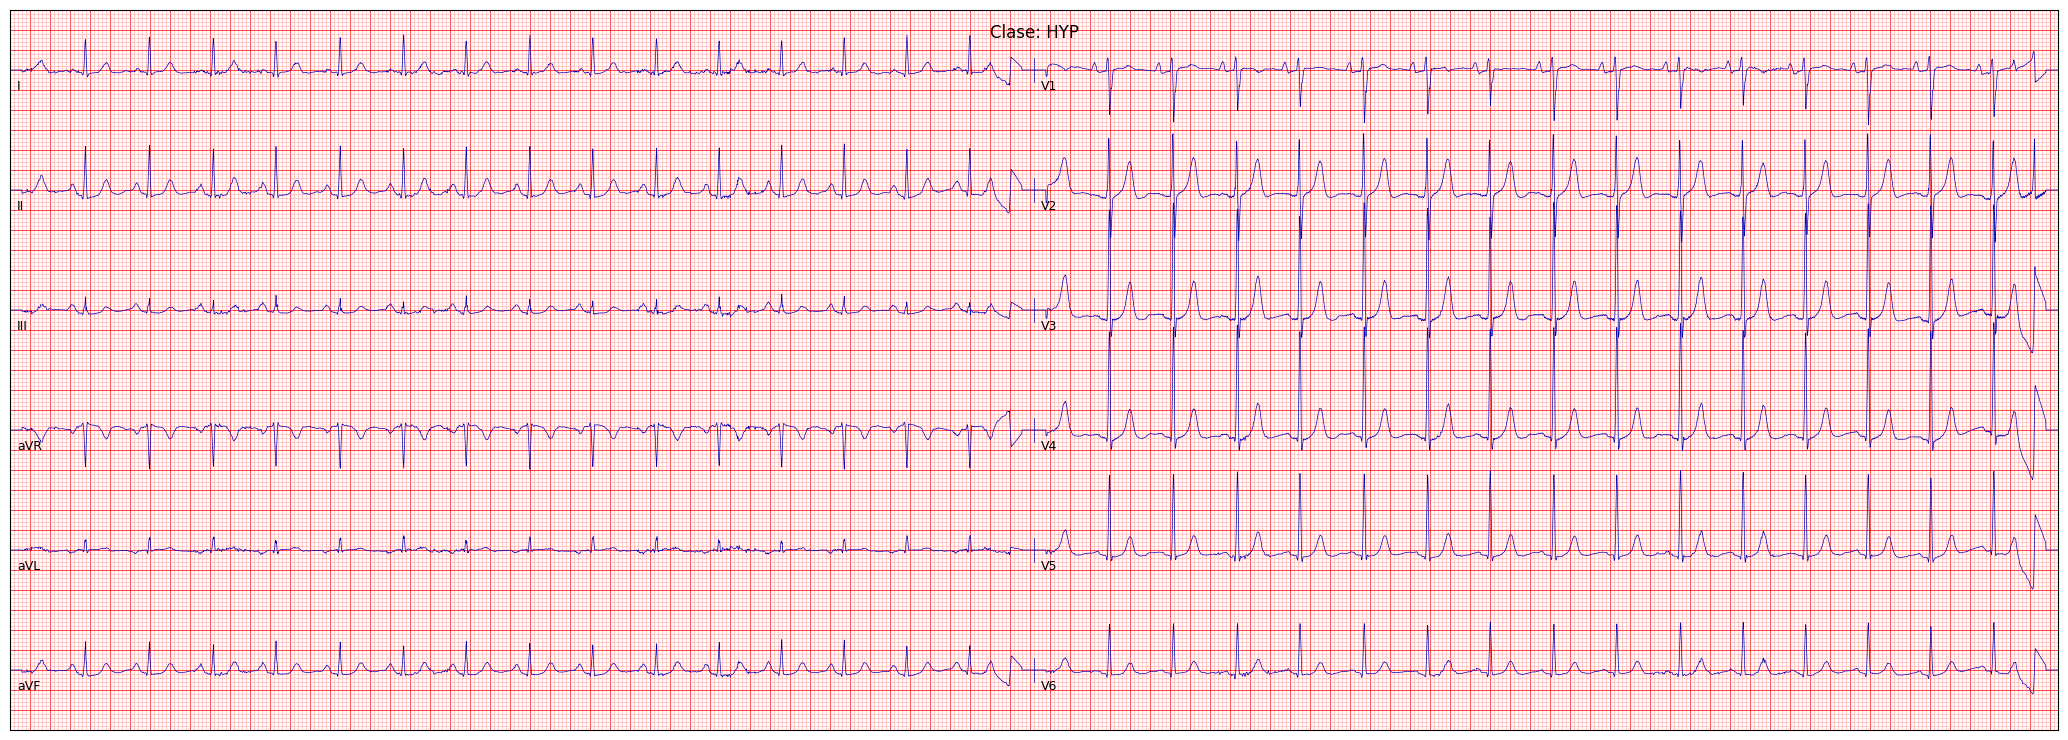
\includegraphics[width=0.9\textwidth]{Imagenes/Vectorial/ECG/HYP.png}
	 	\caption{ECGs de todos los tipos de anomalías.}
	 	\label{fig:ecg_clases}
	 \end{figure}
	
	\subsubsection{Formato de los datos}
	Los ECGs se almacenan en formato WFDB (\emph{Waveform Database}), un estándar ampliamente utilizado en el ámbito médico para almacenar datos de señales anotados \citep{wfdb_spec}.
	
	\subsubsection{Información de pacientes}
	Cada ECG está asociado a información demográfica (edad, sexo, etc.)

En este trabajo únicamente tendremos en cuenta las doce derivaciones del ECG, así como las anotaciones que permiten clasificarlo en una de las cinco etiquetas contempladas en la Sección \ref{subsec:anomalias}.

\section{Modelos para la clasificación de ECG}
\subsection{Enfoques basados en técnicas tradicionales de aprendizaje automático}
El desarrollo de clasificadores ha sido crucial en el campo de la IA enfocada a la detección de anomalías en señales de ECGs. Entre estos métodos, los árboles de decisión y el método k-NN han mostrado una eficiencia notable gracias a su sencillez y capacidad para modelar comportamientos complejos \citep{guo2023machine}.

No obstante, estos enfoques presentan un problema, pues requieren seleccionar de manera manual una serie de características en la señal (como amplitud de la onda R, duración del complejo QRS, etc.), cosa que resulta extremadamente difícil ya que el análisis de electrocardiogramas es muy complejo. Aunque estos métodos resultan efectivos en escenarios con un volumen de datos moderado, su rendimiento depende en gran medida de las características anteriormente mencionadas \citep{acharya_2017}.

\subsection{Modelos basados en redes neuronales}
Las redes neuronales son un modelo computacional inspirado en las neuronas biológicas. Están formadas por capas de neuronas artificiales conectadas entre sí que aprenden a transformar los datos de las entradas en las salidas deseadas. Este aprendizaje se realiza ajustando los pesos de cada conexión, comúnmente mediante el algoritmo de \emph{backpropagation} \citep{backpropagation}, para minimizar un error definido (p.ej., la diferencia entre la salida prevista y la real). De esta forma, en lugar de depender de técnicas de extracción de características diseñadas manualmente, las redes neuronales aprenden internamente los rasgos más relevantes a partir de los datos.

En particular, las CNNs (\emph{Convolutional Neural Networks}, Redes Neuronales Convolucionales) se han popularizado en tareas de visión por computador y análisis de señales al emplear operaciones de convolución (ver siguiente apartado).

Aunque nacieron enfocadas al reconocimiento de imágenes, se han adaptado con éxito a otros tipos de datos, como ondas, usando convoluciones unidimensionales en lugar de bidimensionales. Esto permite a la red detectar características relevantes de la señal (como la forma o duración de los intervalos) sin necesidad de ser elegidas manualmente por un experto, lo que le otorga una gran capacidad de generalización \citep{hannun_cardiologist_2019}.

\subsubsection{Convoluciones}
Una convolución es una operación matemática que toma dos funciones o señales y produce una tercera, mostrando cómo una de ellas “filtra” a la otra. Por ejemplo, en el procesamiento de imágenes, la convolución se utiliza para aplicar filtros o detectores de bordes: se toma una matriz de píxeles (la imagen) y se combina con un kernel (también llamado filtro), multiplicando y sumando los valores de cada posición para generar un nuevo valor en la imagen resultante. Este proceso, repetido a lo largo de toda la matriz, ayuda a resaltar características como contornos o texturas específicas.

En redes neuronales, se utilizan convoluciones discretas (es decir, diseñadas para trabajar con una cantidad de datos discreta, lo que ocurre siempre ya que los datos son finitos) .La convolución es la base para extraer características relevantes de datos de entrada como imágenes o señales (como es el caso de un ECG). Cada capa convolucional aprende pesos que responden a cierto patrón, de modo que, al aplicar esa capa sobre la entrada, se pueden detectar patrones específicos (por ejemplo, la presencia de bordes horizontales o verticales en una imagen). A través de varias capas de convolución, el modelo va construyendo representaciones cada vez más complejas, y eso permite un gran en tareas de clasificación (como es el caso de los ECGs). Esta eficiencia y capacidad de extracción de características es lo que ha convertido a las convoluciones en una herramienta fundamental dentro de la informática moderna, especialmente en los campos de visión por computadora.

\subsection{El modelo de Ribeiro}
Dentro de los enfoques basados en redes convolucionales, destaca el modelo propuesto por \cite{ribeiro}, cuyo objetivo es la clasificación multiclase de ECGs de 12 derivaciones. La arquitectura (que podemos ver en la Figura \ref{fig:ribeiro_arch}) se caracteriza por una serie de capas convolucionales unidimensionales adaptadas a la naturaleza de la señal. Esto permite analizar el electrocardiograma como una señal, sin necesidad de representarla como una imagen.

\begin{figure}[t]
	\centering
	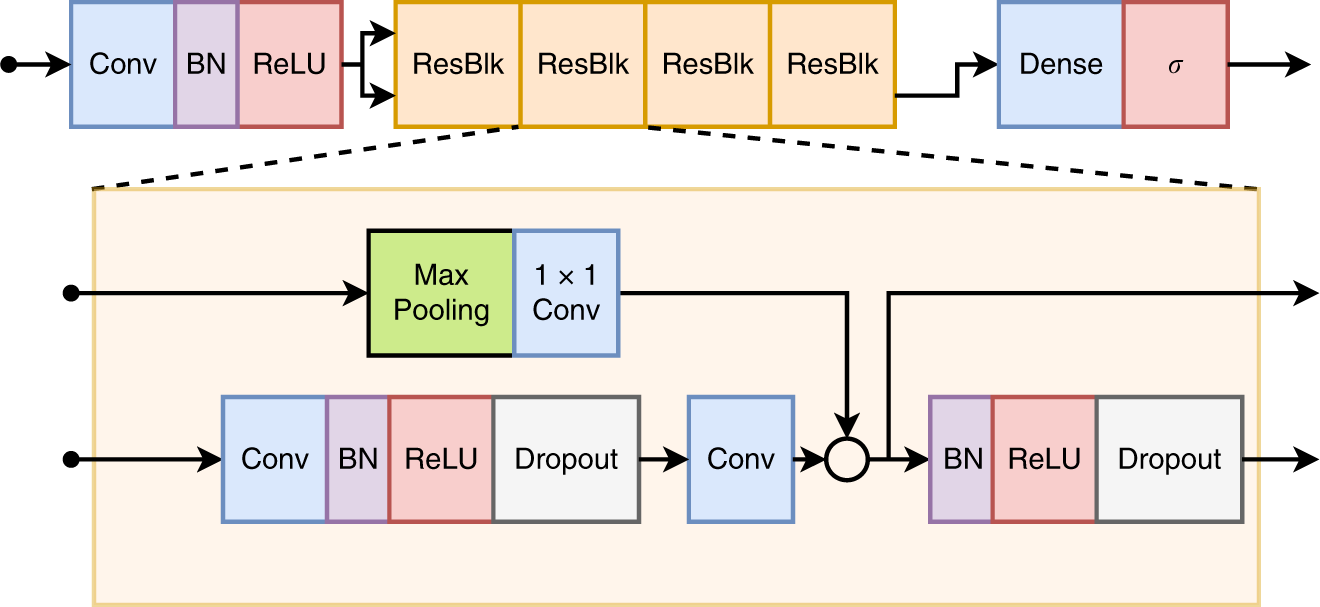
\includegraphics[width=\textwidth]{Imagenes/Vectorial/ribeiro_arch.png}
	\caption{Arquitectura de la red neuronal que se emplea en el \emph{gold standard}. Fuente: \cite{ribeiro}}
	\label{fig:ribeiro_arch}
\end{figure}

Los distintos tipos de capas que utiliza el modelo son las siguientes (para ver más sobre los tipos de capas y su comportamiento completo, el lector puede referirse a \textbf{Deep Learning} \cite{Goodfellow-et-al-2016}):

\begin{enumerate}
	\item \textbf{Conv}: Las capas convolucionales mencionadas anteriormente.
	\item  \textbf{BN}: Son capas de \emph{batch normalization}, que mejoran y aceleran el entrenamiento.
	\item \textbf{ReLU}: Capas de activación, que devuelven 0 si el valor de la entrada es negativo.
	\item \textbf{Dropout}: Una capa que desactiva un porcentaje aleatorio de las neuronas en cada entrenamiento, para evitar ciertos problemas como la sobrespecialización.
	\item \textbf{Max Pooling}: Se utiliza para reducir la dimensionalidad de la entradda.
	\item \textbf{Dense}: Esta capa se suele utilizar antes de una función de activación para adecuar el número de salidas del problema
	\item \textbf{$\sigma$}: Capas sigmoides, transforman la salida de las neuronas en un valor real entre 0 y 1. Son útiles para acotar la salida.
\end{enumerate}

Como puede verse en el artículo de \cite{ribeiro}, el modelo demostró un alto desempeño en la detección de diversas anomalías. En este trabajo, adaptaremos ligeramente la capa de entrada de este modelo para poder tomar como entrada matrices de cualquier tamaño (originalmente el modelo requería de matrices de dimensión 12xN) para poder entrenarlo con transformaciones de la señal original a imágenes. Sin embargo, no modificaremos la estructura interna de las capas convolucionales.

\section{Explicabilidad en la IA}
A pesar de que los modelos de \emph{Deep Learning} han demostrado su eficacia en tareas de diagnóstico clínico, es necesario contar con métodos que ofrezcan explicaciones y permitan interpretar sus predicciones, ya que la actual legislación europea (\href{https://europa.eu/youreurope/business/dealing-with-customers/data-protection/data-protection-gdpr/index_es.htm}{\emph{GDPR}}) exige poder dar una explicación comprensible de cualquier decisión tomada por un algoritmo o modelo predictivo. Esto es particularmente relevante en el ámbito médico, donde cualquier decisión que tome un algoritmo debe poder justificarse ante profesionales de la salud, ya que la salud de una persona podría verse afectada por esta decisión.

Algunos de los métodos más notables de explicación en la IA son los siguientes:

\subsubsection{Métodos intrínsecos}
Estos métodos consisten en analizar el código del modelo de IA para comprender qué hace exactamente un modelo por dentro. Estos métodos solo son aplicables cuándo el el modelo es intrínsecamente explicable, es decir, que hay una clara correlación entre el código del modelo y la salida del mismo, como es el caso de los árboles de decisión o regresiones lineales.

Las redes neuronales no entran dentro de este tipo de modelos, y por tanto no podemos aplicar este tipo de explicaciones en este trabajo.

\subsubsection{Métodos basados en visualización}
Estos métodos consisten en representar gráficamente qué partes de la entrada son más relevantes a la hora de tomar una decisión. Por esto, están estrechamente relacionados con el significado de los datos de entrada, y no tanto con su forma. Supongamos que tenemos como entrada una matriz de dos dimensiones. Esto puede interpretarse (entre otras cosas) como una imagen o como una serie de vectores de mediciones distintas (esto último se conoce como serie temporal) en el tiempo:

\begin{itemize}
	\item Si los datos representan imágenes, existen métodos como Grad-CAM para dibujar mapas de calor sobre la imagen original que señalan las partes más relevantes de la imagen a la hora de tomar decisiones.
	\item Si tenemos una serie temporal, para explicar qué zonas son más importantes lo que necesitamos es señalar, en cada una de las mediciones, qué franjas temporales son más relevantes para la decisión. Esto es lo que hacen algunos métodos como \emph{saliency maps}.
\end{itemize}

\par

Si bien es cierto que en este trabajo tenemos tanto series temporales (los datos originales sin transformar) como imágenes (los datos transformados), en este trabajo utilizaremos exclusivamente \emph{saliency maps}, por motivos que veremos en el Capítulo \ref{cap:explicabilidad}.

